\clearpage
\section{考察}
\begin{enumerate}[1.)]
	\item 各設定に対して,横軸が電流,縦軸が電力のグラフ(一つにまとめる)を描け.
	\begin{figure}[h]
	\centering
	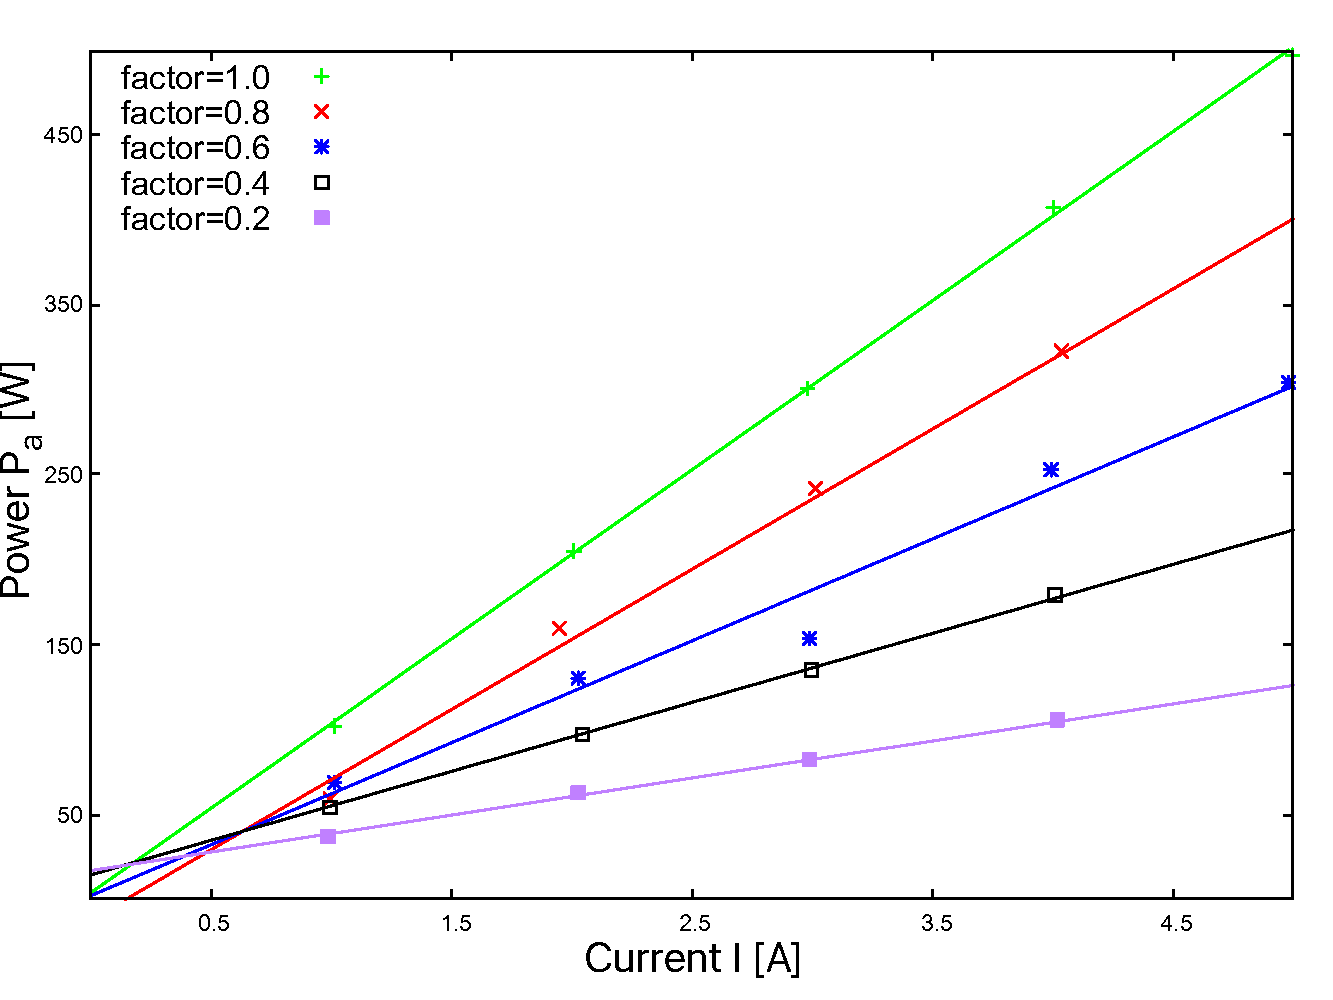
\includegraphics[scale=0.6]{./data/L/L.pdf}
	\caption{$X_L$の電流-電力特性}
	\label{fig:L}
	\end{figure}
	\begin{figure}[h]
	\centering
	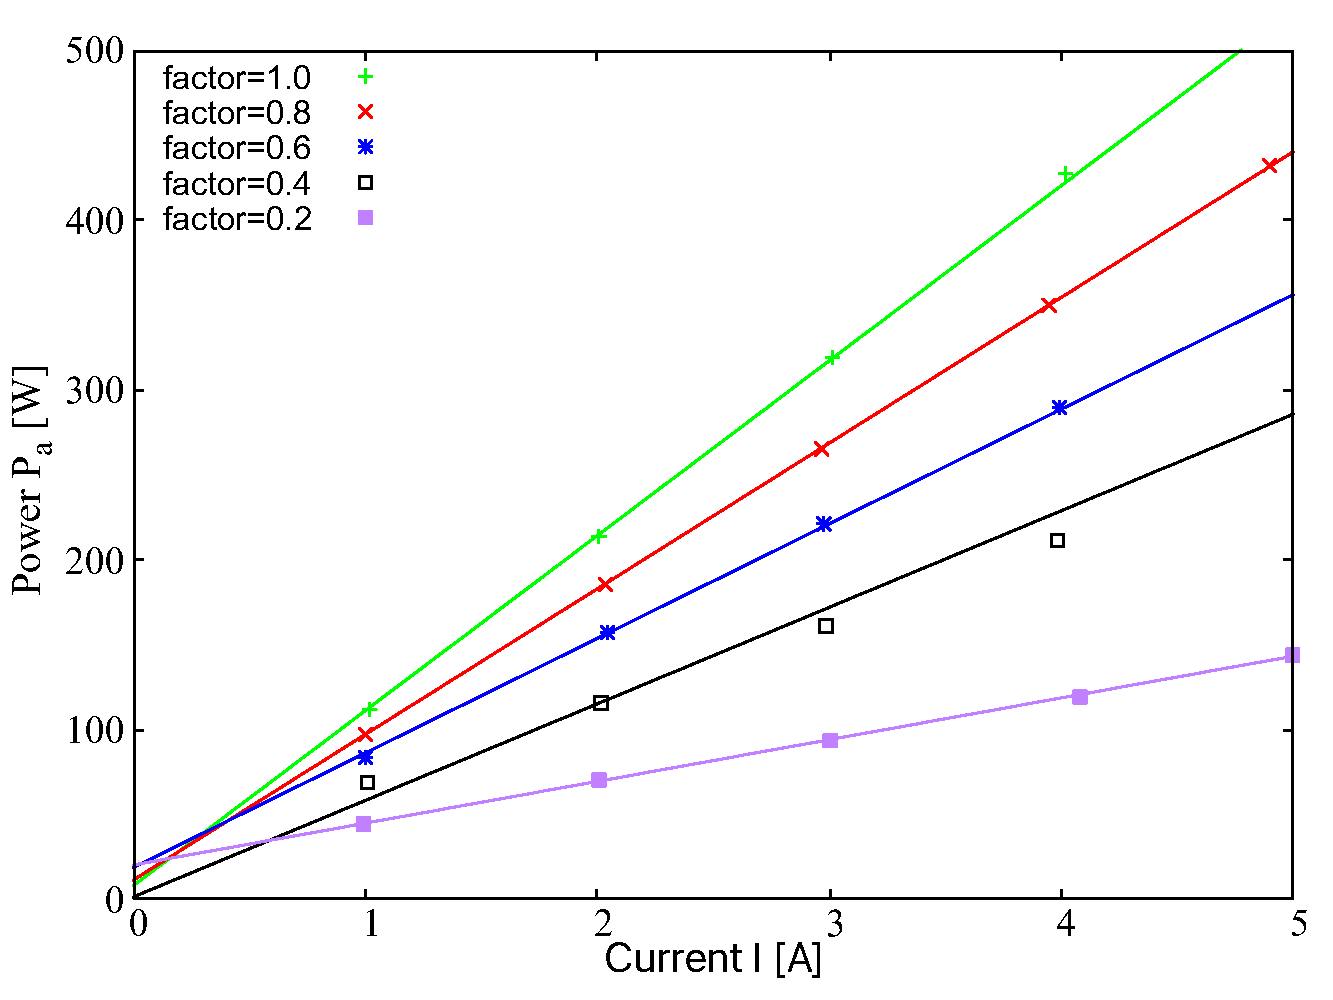
\includegraphics[scale=0.6]{./data/C/C.pdf}
	\caption{$X_C$の電流-電力特性}
	\label{fig:C}
	\end{figure}
	\item 各電流計の指示に対して,横軸が力率,縦軸が電力のグラフ(一つにまとめる)を描け.
	\item 電力と電圧,電流,力率の関係を述べよ.
	\item 
\end{enumerate}